\chapter{Introduction}

\label{chpt:Chapter1}

\chapterauthor{Nikolai G. Vetr}

%\AddToShipoutPictureFG*{\put(-15,-27){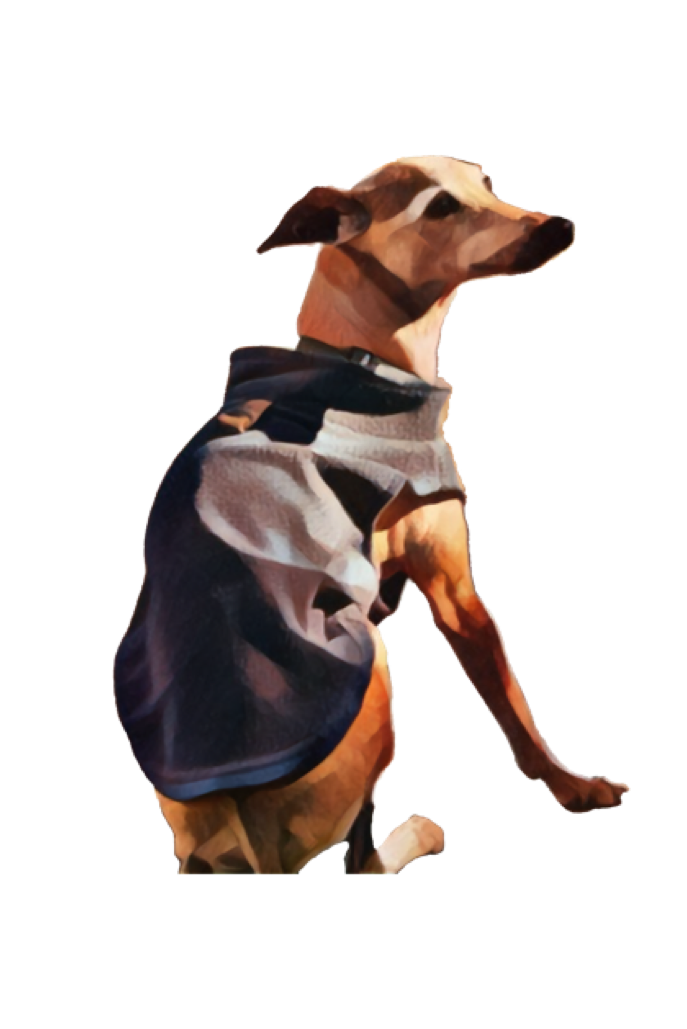
\includegraphics[width=40mm,scale=1]{figures/pooper.png}}}


\clearpage


\section{The Need for Phylogenetic Models of Morphological Evolution}

Biological variation both in the extant and fossil records is the outcome of a wide array of evolutionary and non-evolutionary processes. Darwin's ``endless forms most beautiful'' \citep{darwinOriginSpeciesMeans1859} emerge proximally from the complex interplay of environment and development, but ultimately owe the bulk of their between-group differences to millions and billions of years of chance intergenerational sampling effects and reproductive asymmetries attributable to the heritable underpinnings of those organisms' morphology, physiology, behavior, biochemistry, and other traits \citep{mayrNewPhilosophyBiology1988}. Coupled with the bifurcating process by which reproductive isolation emerges and permits populations to proceed along independent evolutionary trajectories, we see these forms --- these \textit{species} --- emerge and change, contract and die. By examining that variation and imagining a description of the processes that might have generated it, we can make inference of phenomena beyond the remit of immediate observation and guess at not just the tempo and mode of character evolution driving within-lineage variation, but also the order and timing of splitting events that birthed those series of independent daughter lineages. 

We can represent an estimated history of these splitting events with a tree, be it one of population history (in the case of groups at the sub-specific level) or phylogeny (for group at or above the species level), which can be rooted to specify the order of events through time, or unrooted, as a means of constraining that order. With a mathematical description --- or stochastic model --- of the evolutionary process that changes the states of characters along branches of the tree, we can predict what sorts of observations we might expect to make at the tips of our tree, and explore how varying properties --- parameters --- of our tree and stochastic model might affect the distributions of those predictions. Comparing our real-world observations with the fictitious ones predicted by our model, we can find combinations of parameters more or less consistent with what we observe. The more plausible our data look under some instantiation of our model parameters, the better evidenced we might say those parameters are, allowing us to discriminate between alternative phylogenetic hypotheses. Through straightforward manipulation of the definition of conditional probability, we can combine a function describing the plausibility of our data with one describing the prior probability of our model parameters to strike a compromise between them, learning what probability we should ascribe to different hypotheses after having made our observations \citep{bayesLIIEssaySolving1763}, at least to the extent that we are willing to accept as given the assumptions of our data-generating process.

If our model is a poor representation of the evolutionary processes that give rise to variation, neither plausible nor probable model parameters may be very trustworthy. Tremendous efforts have gone into developing models to describe the evolution of molecular characters, of nucleotides, amino acids, proteins \citep{hollandRiseStatisticalPhylogenetics2013, kapliPhylogeneticTreeBuilding2020}, but comparably little attention has been paid to models of morphological evolution, especially of the hard tissues that preserve especially well in paleontological contexts. And while neontologists make ample use of increasingly sophisticated methods to infer phylogeny among extant taxa, those reliant on morphology must make do with either heuristic methods lacking in flexibility or other desirable properties \citep[e.g. a principled accounting of inferential uncertainty, consistency at the limit of infinite data, etc.]{wrightBayesianAnalysisUsing2014}, or else fit models of character evolution that make uncomfortable assumptions about the nature of morphological evolution \citep[e.g. independence between characters, monomorphism within lineages, etc.]{felsensteinInferringPhylogenies2004}. And where more sophisticated models exist, their implementation might be sufficiently inefficient as to render practical inference a distant pipe dream, so slow as to be called computationally intractable. 

The work presented in this dissertation does not claim much in way of novelty --- the models contained herein have been known for many decades --- but it does develop a few small tricks that make fitting certain stochastic models more practically efficient under the limits of modern computer hardware, as well as a few novel means of visualizing and interpreting those fitted results. In this manner it extends past work \citep[as e.g.][before it]{felsensteinMaximumlikelihoodEstimationEvolutionary1973, felsensteinUsingQuantitativeGenetic2005}, much as past work made more practical previously proposed methods and theory. Likewise, it does not address every complaint in the matter of biological realism levied against popular models of morphological evolution. But it does explore the statistical properties of some of the more satisfying models under consideration, both on their own merits and in comparison to alternatives. Occasionally, it shifts its attentions away from its primary focus, the set of branching events collectively called the phylogenetic tree's \textit{topology}, and towards other aspects of the phylogenetic model, such as variation in evolutionary rates between characters, across lineages, or through time, or reconstructions of character histories, in the case of truncated biogeographic diffusions. Most of its empirical focus lies with extant humans and close relatives for whom phylogenies and population histories are well-resolved, or at least halfway understood, that more experimental inferential methods may be evaluated by reference to molecular expectation. The primary model considered here is that of multivariate Brownian motion (mvBM), acting either on raw or log-transformed character data, on a vector subspace of that data, or on that data after its been passed through an ordinal probit discretization filter. The mvBM model can be derived under quantitative genetics to correspond a broad range of composite evolutionary processes \citep{hansenTranslatingMicroevolutionaryProcess1996}, and it is exceptionally easy to work with, making it an excellent target for exploratory phylogenetic study. An overview of the broader class of evolutionary models to which it belongs, as well as motivations for using this model over others, can be found in the section below.

\clearpage

\section{A Brief Overview of Popular Continuous Character Evolutionary Models}

\subsection{Ornstein-Uhlenbeck Processes}

Brownian motion can be thought of as nested in another, more parameter-rich model of character evolution called the ``Ornstein-Uhlenbeck'' process \citep[OU]{butlerPhylogeneticComparativeAnalysis2004, beaulieuModelingStabilizingSelection2012}. This process resembles Brownian motion, except it incorporates an elastic, centripetal force by which quantitative traits are pulled toward some optimum value $\theta$ with magnitude of pull proportional to their distance from $\theta$ and a “strength of selection” parameter $\alpha$. Where under Brownian motion  the change a trait underwent in a single time step is state-independent, under OU it depends on the current state, such that $X_{t+1}$ = $X_t$ + $\alpha$($\theta$ – X$_t$) + N($\mu$,$\sigma$), or dX$_t$ = -$\alpha$(X$_t$ - $\theta$)dt + $\sigma$dBt \citep{hansenStabilizingSelectionComparative1997}. If X$_t$ is greater than $\theta$, $\alpha$($\theta$ – X$_t$) will be negative and the trait in the next time step will be pulled “downwards” (proportional to the strength of selection coefficient $\alpha$). Conversely, if $X_t$ is less than $\theta$, X will be pulled upwards in the next time step. Brownian motion, then, arises as an Ornstein-Uhlenbeck process where $\alpha$ is 0. Traits are expected to evolve toward the $\theta$ until they reach it, after which they will fluctuate around it without ever straying too far (Figure \ref{fig:OUPonds}a). The larger $\alpha$ is, the faster traits will reach the optimum and the less they will fluctuate around it. A greater variance in the Brownian motion component of the Ornstein-Uhlenbeck process (i.e. a higher $\sigma$), meanwhile, will increase variance among the traits, leading to non-identifiability when trying to infer the values of $\alpha$ and $\sigma$ from tip data, since an increase in one can be largely counteracted by an increase in the other. 
 
Though the Ornstein-Uhlenbeck process does provide a measure of biological realism, it poses certain additional difficulties to the inference of phylogeny itself, difficulties that may render attempts to use it to retrieve model parameters such as tree topology futile. Under univariate OU with a single peak, the distribution of continuous character states at time $t$ for a character with starting value X$_0$ is normal, with mean $\theta + e^{-\alpha t}(X_0 - \theta)$ and variance $\sigma^2(1-e^{(-2\alpha t)} / (2\alpha)$. From this, it is easy to see that as $t$ increases, the expression $e^{-\alpha t}(X_0 - \theta)$ goes to 0, and the long-term behavior of X centers around $\theta$, with variance determined by our two non-identifiable OU model parameters $\alpha$ and $\sigma$. Effectively, this limits the extent to which the signature of shared ancestry can persist in realizations from an OU-process at the tips of a tree. After sufficient time has passed, all tip values sample from the same, independent distribution determined by $\theta$, $\alpha$ and $\sigma$, which is to say there no longer exists information about between-tip character covariation due to shared ancestry in those values. Rather than phylogenetic covariances decreasing linearly with phylogenetic distance, they instead increase exponentially \citep{hansenTranslatingMicroevolutionaryProcess1996}. Conversely, if $\alpha$ or $t$ are sufficiently small, such as when characters are far from their soft limits in state-space over the timescales represented in the phylogeny, the OU process resembles a Brownian motion process, for which there exist more convenient and tractable multivariate likelihood functions as described later in this work (Chapter \ref{chpt:Chapter2} and Appendix \ref{app:App1}). 

To summarize, then: the more a single-peak OU process is needed to describe the character evolutionary process, the less useful realizations from that process will be for phylogenetic inference. For our purposes here, it may be best to first understand the extent to which Brownian motion, in its best-case context of little-to-no model misspecification, performs, leaving for others a greater detail exploration of those contexts in which an OU model breaks down when used to infer phylogeny. Additionally, a single-peak OU process may itself be a poor fit to the data, for which reason we might wish to posit the existence of multiple peaks. But adding peaks also adds parameters whose inference of marginalization is necessary, potentially robbing us of the power necessary to infer phylogeny and complicating our computations greatly. And at the limit, we might wish to specify as many peaks as we have independently evolving lineages, and further relax the assumption that these peaks' locations be static through time, perhaps allowing them to wander themselves in a manner analogous to fluctuating selection. But such a complex model strongly resembles a laggy Brownian motion, and indeed collapses to Brownian motion at sufficiently high $\alpha$ \citep{hansenTranslatingMicroevolutionaryProcess1996}. Similarly, uncorrelated selection models (where the magnitude and direction of selective effects are sampled from some background distribution, typically normal, across time steps) and directional selection models (where all lineages share the same selective pressures) can also be shown to be equivalent to a Brownian motion model under certain conditions \citep{hansenTranslatingMicroevolutionaryProcess1996}.

This is not to say that OU-models are not useful, especially within their more usual role, serving as a candidate model in the phylogenetic comparative method. In work done in association with this dissertation but outside its scope, I explored their application in Stan for predicting reactive nitrogen concentrations across a hierarchically structured set of manure ponds across California (Figure \ref{fig:OUPonds}). But their use here is limited, and so they shall not be considered further.

\begin{figure*}[h]
\centering
\includegraphics[width=160mm]{figures/OU_Ponds.pdf}
\caption[Posterior Predictive Distribution of a Hierarchical OU Model]{In a), realizations from an OU process over 4 days for Pond 17, averaging over posterior uncertainty. Mean values for all univariate OU model parameters are labeled, with samples from the posterior distribution for $\theta$ marked in red. The joint posterior distribution can be sampled and simulated from to generate posterior predictive distributions for arbitrary timepoints, marked with blue dashed lines. In b), kernel density plots of these posterior predictive distributions are provided, with corresponding timepoints labeled. A final timepoint, t$_\infty$, gives the limiting distribution for the process. The model used here was a hierarchical model, and could be analogized to a star phylogeny of manure ponds whose optima evolve on the tree according to a Brownian motion process, with returning force ($\alpha_i$) and rate ($\sigma^2_i$) parameters for each pond$_i$ estimated according to exponential hyperdistributions for each. \label{overflow}
\label{fig:OUPonds}}
\end{figure*} 

\subsection{Morphological Clock Models}
 
Another common modification made to the Brownian motion process in phylogenetic comparative contexts involves an allowance for the rate parameter to vary through time \citep{blombergTestingPhylogeneticSignal2003, harmonEarlyBurstsBody2010}. Specifically, one may set the Brownian motion rate parameter at time t ($\sigma^2_t$) equal to a product of the initial rate ($\sigma^2_0$) and the base of the natural logarithm (e) raised to the power of the product of some constant (r) and time (i.e. $\sigma^2_t$= $\sigma^2_0 e^{rt}$). If r is negative, rates will start off small and increase through time, leading to an Accelerating (AC) or Late Burst (LB) model of trait evolution. Meanwhile, if r is positive, rates will start off large and decrease through time, leading to a Declining (DC) or Early Burst (EB) model of trait evolution. If r is 0, the ACDC / Burst model collapses back into standard Brownian motion, as $e^{0t} = 1$ and $\sigma^2_t$ = $\sigma^2_0$. The inclusion of this extra layer, then, allows you to fit models that capture hypotheses pertaining to rapid diversification of form following a lengthy stasis, or vice versa. 

In practice, phylogenetic likelihood calculation under these relaxed clock models works by rescaling the branch lengths of a phylogeny according to the integral of the rate function along each branch. This consideration reveals that all these named variations on Brownian motion should not \textit{properly} be thought of as different character evolutionary models at all, but rather different \textit{clock} models, relaxations on the assumption of a strict morphological clock dictating proportionality between morphological evolution and either time or molecular evolution. So too should be considered other transformations of phylogenetic branch lengths, such as Pagel's $\lambda$, $\kappa$, and $\delta$ \citep{pagelMaximumLikelihoodApproach1999, pagelInferringHistoricalPatterns1999}, which are often interpreted to respectively measure ``phylogenetic signal'' (i.e., as an informal test of the strict morphological clock), association between diversification rate and morphological change, and more gradually slowing or speeding rates of evolution. For our purposes here, we typically place no strong constraints on variation in the rate of the morphological clock throughout a tree, preferring instead to set weakly informative, regularizing priors on branch lengths. As most of the analyses that follow lack an independent or jointly performed estimate of phylogeny on which morphological rate variation could be meaningfully considered, we instead infer trees whose branch lengths are in units of the square root of expected morphological change (specifically, the variance, $\sigma^2$ of a particle under Brownian motion scales linearly with branch length, and its expected absolute deviation can be found by evaluating twice the integral of the normal probability density function across (0, $\infty$), which equals $\sigma \sqrt{2 / pi}$). 

As in the preceding section, work done in association with but outside the strict scope of this dissertation explored our ability to retrieve parameters of relaxed morphological clocks --- for example, centering an evolutionary burst not at the root of the tree, but some distance into its branches. Here, we examined the role mass extinction events (specifically the Cretaceous–Paleogene) played in the evolution of fish feeding morphology (Figure \ref{fig:middleBurst}). In addition, a short simulation study identified the effects of such a ``middle-burst'' on disparity through time \citep{harmonTempoModeEvolutionary2003} plots (Figure \ref{fig:disparityThroughTime}), a heuristic and difficult-to-interpret attempt to capture phylogenetic rate variation.
 
\begin{figure*}[h]
\centering
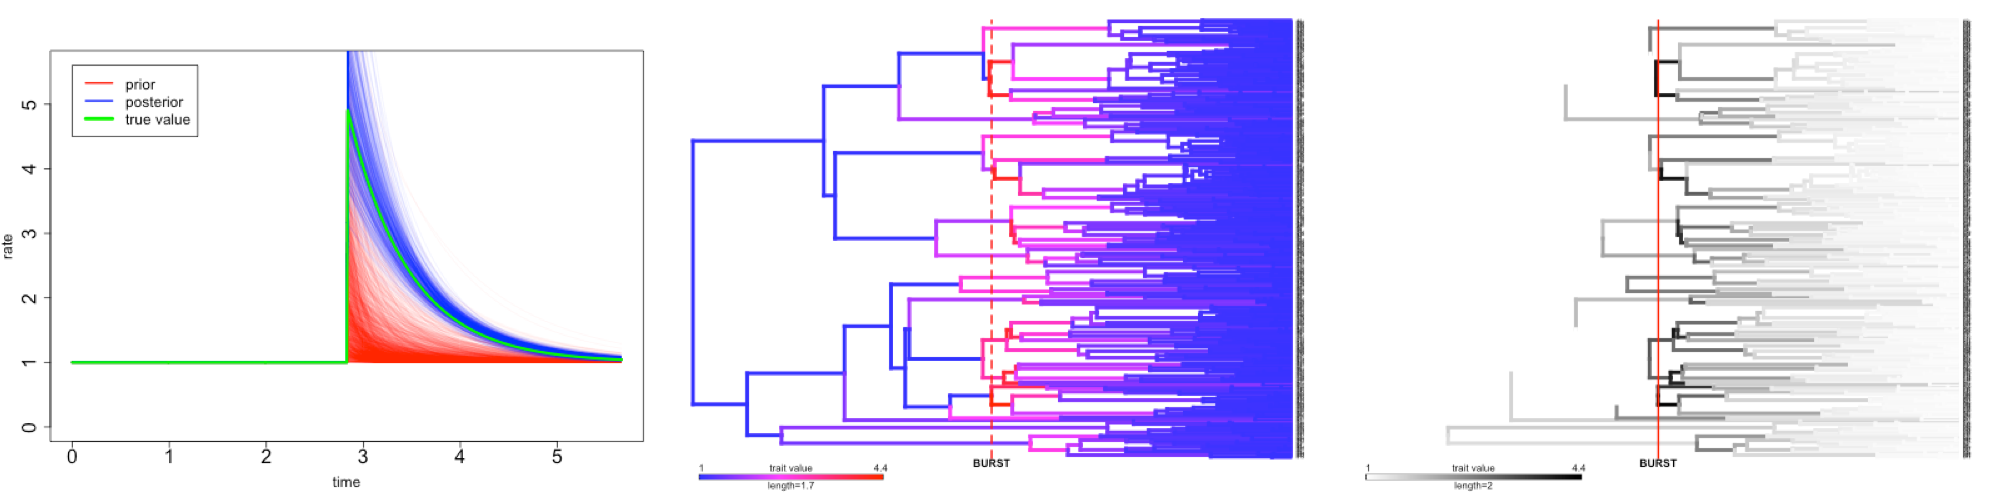
\includegraphics[width=160mm]{figures/middle_burst.pdf}
\caption[Posterior Distribution of a Middle Burst Brownian Motion Model]{The result of a single simulation experiment attempting to infer the magnitude and decay constant of an evolutionary burst of known location given a known tree with 450 tips and univariate character data. In a), samples from both the prior and posterior are plotted and labeled, with the true value of the burst shown in dark blue. In b-c), branch-rates are plotted on the phylogeny used with color-coding and on a white-black gradient, respectively. 
\label{fig:middleBurst}
\label{overflow}}
\end{figure*} 

\begin{figure*}[h]
\centering
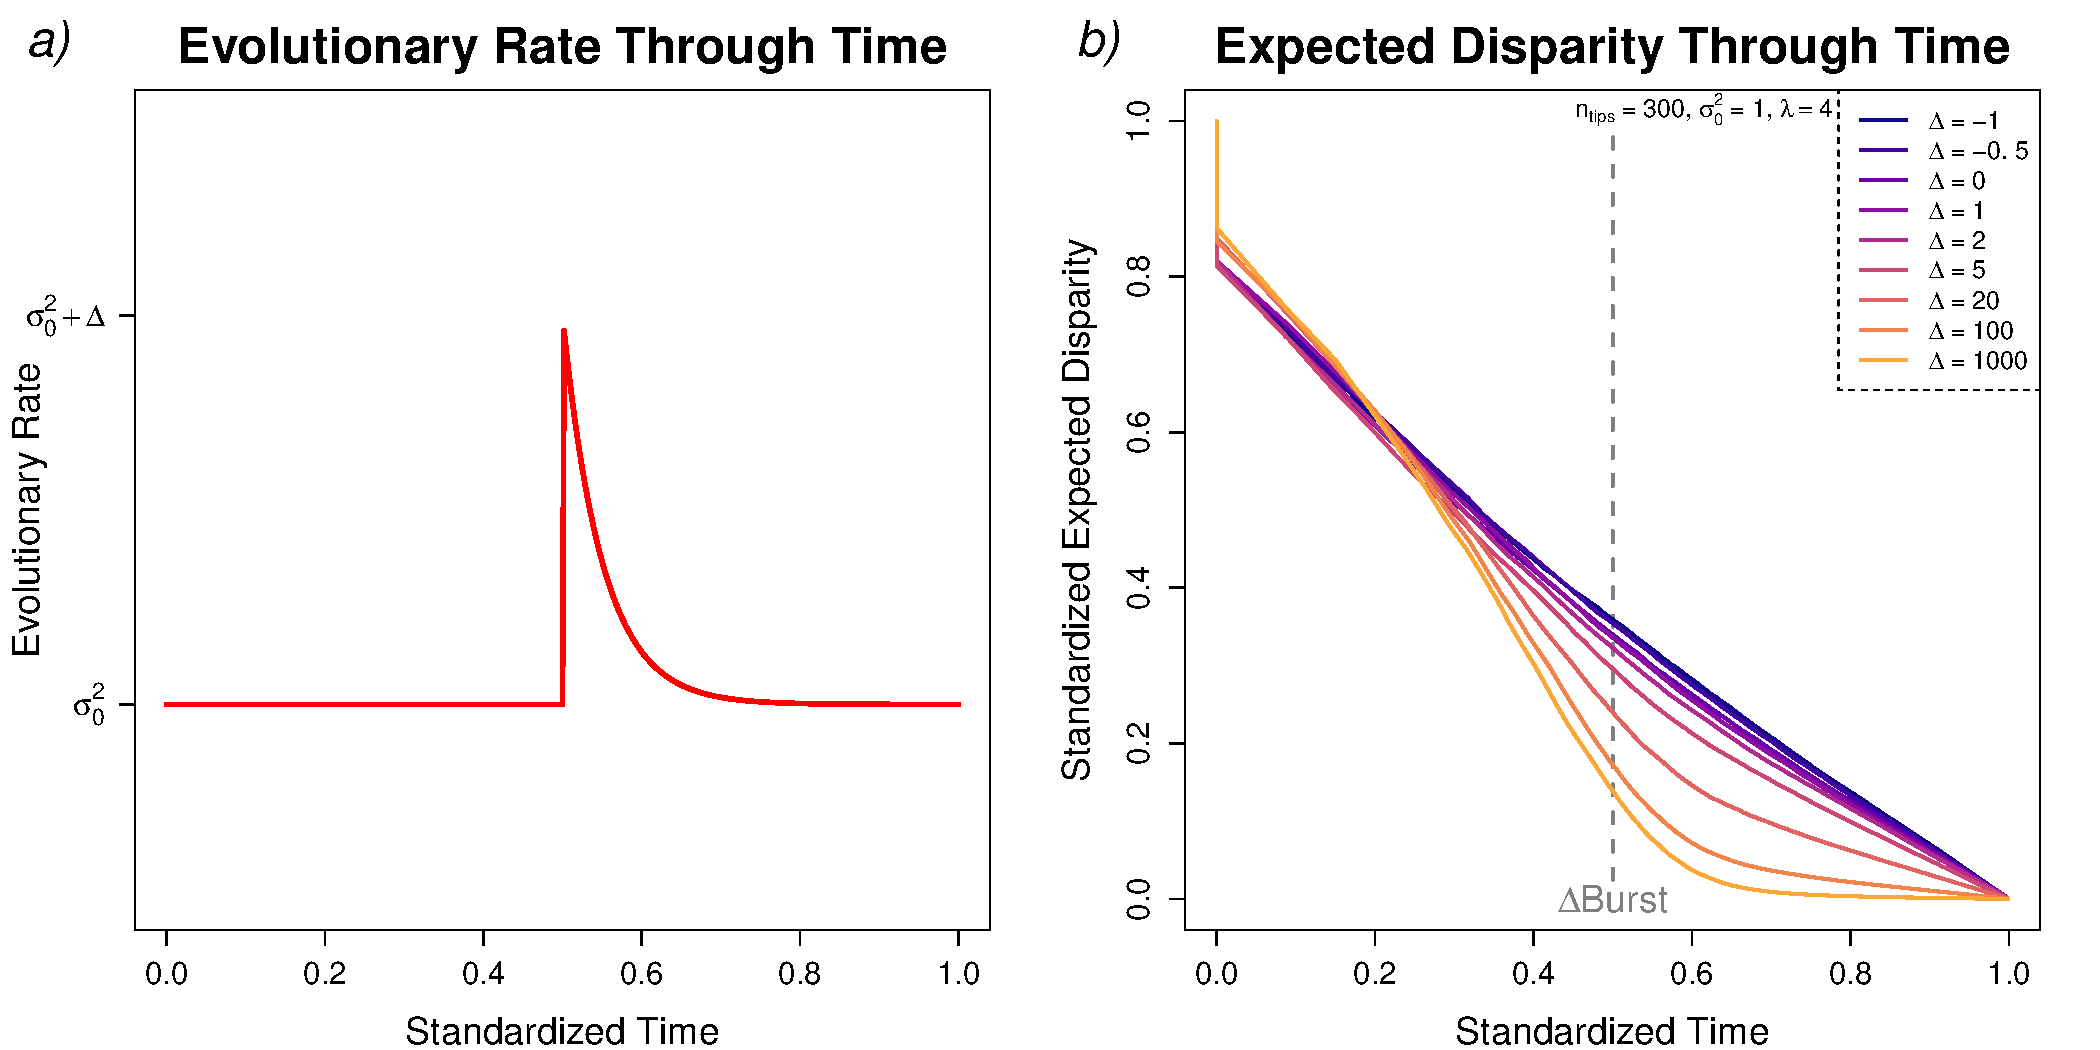
\includegraphics[width=160mm]{figures/expected_disparity_through_time.pdf}
\caption[Variation in Expected Disparity Through Time Under Varying Middle Bursts]{An exploration of the expected trend of a disparity through time plot for a tree with 300 taxa. In a), the relaxed morphological clock model is shown, featuring a change in evolutionary rate at the temporal middle of the tree, followed by an exponential decay to normalcy. The magnitude and direction of the change is given by $\Delta$, and expected trends for different values of $\Delta$ are shown in panel b). 
\label{overflow}
\label{fig:disparityThroughTime}}
\end{figure*} 
  
%Figure 3. 50 independent replicates for both an Early Burst and a Late Burst process over 100 time steps with a starting state of zero. In the Early Burst model, r was -0.05 and the starting rate was 100; in the Late Burst model, r was 0.05 and the starting rate was 1. 

\clearpage

\section{Benefits of Working in a Bayesian Inferential Framework}

Model-based inference is preferred in part because of the flexibility it affords --- should something in the set of considered models dissatisfy, it can be straightforward to engineer a better model, one more able to capture the suspected underlying biology responsible for generating empirical data. But having committed ourselves to the likelihood principle, we encounter a further dilemma: should the model be fitted in a (penalized) Maximum Likelihood framework, searching for the most plausible set of model parameters? Or should we instead try to reach a compromise between the information contained within our data, as perceived by our likelihood function --- and our prior beliefs about the probabilities of different model parameters? As the title of this work suggests, we generally opt for the latter strategy, carrying out most inference in a Bayesian framework. This is despite objections raised by both those in favor of Bayesian approaches \citep{gelmanHolesBayesianStatistics2020} and those out of favor \citep{gelmanObjectionsBayesianStatistics2008}. Our motivations in these regards are many and are described below:

\paragraph{Interpretability}

Though Bayes' theorem is, at heart, a trivial implication of introductory probability theory, it provides an elegant, powerful, and necessary vehicle by which to obtain probabilistic estimates of model parameters. Most scientists' statistical intuitions naturally hew close to Bayesian interpretations of probability \citep{kaplanNullRitualWhat2004}, and accommodating inferential uncertainty and evaluating the degree of support in the data for competing hypotheses is much simpler with a probability than with devices such as the non-parametric bootstrap \citep{efronBootstrapMethodsAnother1979, felsensteinConfidenceLimitsPhylogenies1985}. When prompted, most practitioners default less to thinking in terms of sampling distributions of estimators and more to interpreting p-values or bootstrap support estimates as probabilities of alternative hypotheses \citep{greenlandStatisticalTestsValues2016}. Performing the non-parametric bootstrap in a multivariate framework would also require additional data transformation before resampling, as any data resampled with replacement would necessarily be perfectly correlated with itself, incapable of contributing additional phylogenetic information.

\paragraph{Prior Information}

Though often viewed as a detriment, Bayesian inferences allows for the incorporation of prior information into our analyses, forcing us to explicitly encode our beliefs about the model in greater detail than just those assumptions implicit to our choice of likelihood function (equivalent to point-mass priors on parameters of some higher nested model). We can specify prior distributions on model parameters as informatively or uninformatively as we feel justified, and further evaluate the extent to which results are sensitive to our choice of priors by running the model under different combinations of prior distributions and contrasting the resultant posterior distributions. When analyzing data, we rarely think that all possible supported parameter values are equally plausible: trees are unlikely to be a trillion units long, and evolutionary rates probably will not vary by dozens of orders of magnitude. Why \textit{not} incorporate this prior information into our analysis in the most principled possible way?

\paragraph{Regularization}

Beyond, encoding our prior beliefs about the data-generating process, priors also serve an important role in preventing undue excitation of the likelihood function in regions of parameter-space that fit especially well to the data, despite not being intrinsically plausible. In so doing, priors help us to tread the line between overfitting and underfitting, balancing error resulting from the model learning from noise in the data with error from the model being insufficiently flexible. In phylogenetics, priors can help us tease apart otherwise non-identifiable parameters whose combination forms a ridge in the likelihood surface, such as clock rates and time during divergence time estimation. They also help us to avoid capture of the model by singularities in that surface, such as when estimating both the value and parameters of a normally distributed random variable (for example, if jointly estimating tip states and the branch lengths separating them under Brownian motion). Hierarchical model structure also lets the model itself learn how skeptical it should be about extreme parameter values, adaptively regularizing priors only to the extent justified by the data \citep{gelmanWhyWeUsually2012}. This strategy finds extensive application in other work, including non-phylogenetic side projects performed in association with this dissertation, but is also used in the catarrhine landmark and discrete dental analyses to flexibly tune the amount of rate variation between traits and branches permissible in those applications. In this manner, we allow the model to partially pool information between parameters, lending aid from highly concentrated regions of the joint posterior to those more diffuse. Though less of a concern in phylogenetic applications, adaptive regularization also helps us to avoid multiple comparisons problems \citep{gelmanWhyWeUsually2012}, such as when we do inference over dozens of rates and examine the ones assessed to be more or less confidently determined.

\paragraph{Stability}

In cases where the likelihood surface is multimodal, Bayesian inference may more easily traverse the distance between peaks than a stochastic optimization algorithm, arriving at more robust estimates of model parameters than mere search for phylogenetic optima. When performing empirically parameterized simulation studies, sampling from the posterior distribution of an analysis of real-world data also helps to better represent the problematic nature of real-world data than the idealization of trees samples from parametric distributions or the simulation invariance of using a single phylogenetic Maximum Likelihood Estimate (MLE). As we use numerical algorithms to approximate joint posterior distributions, we also find ourselves endowed with the tools to assess their reliability. A purported MLE might actually represent a local maximum, with little diagnostic recourse but to compare the output of multiple independent runs, but MCMC output can be screened with many devices to ensure healthy chain mixing and convergence over and on the target distribution.

\section{Prospectus}

A table of contents appears at the start of this work, but it is also fitting to describe what is to come in prose. The ultimate goal of this work was to adapt the threshold model of quantitative genetics to the purpose of inferring phylogeny, and in particular the topologies of trees scaffolding the evolution of high-dimensional ordinal character data (Chapter \ref{chpt:Chapter4}). The primary empirical application of this work was an alignment of ordinal dental traits codified in the Arizona State University Dental Anthropology System \citep{turnerScoringProducesKey1991} and collected by Dr. Shara Bailey. Before that could be done, we first needed to develop and implement a multivariate Brownian model of character evolution, as well as explore its statistical properties in simulation (Chapter \ref{chpt:Chapter2}). Here, we applied the method to a publicly available, open-source dataset of craniofacial linear measurements collected by William W. Howells \citep{howellsCranialVariationMan1973, howellsSkullShapesMap1989, howellsWhoWhoSkulls1995}. In between these, we also compare the performance of our multivariate Brownian motion model to a menagerie of methods commonly used to infer phylogeny using morphology on a cranial landmark dataset collected on 13 different species of catarrhine primate by Katerina Harvati (\citeyear{harvatiNeanderthalTaxonomyReconsidered2004}) and colleagues (Chapter \ref{chpt:Chapter3}). Trees from these analyses could be compared to a well-resolved reference tree obtained from a published analysis of molecular data \citep{arnold10kTreesWebsiteNew2010}, that the yardstick of method performance not be exclusively fictitious, in the sense of agreement with some simulated ground-truth, but also relate in some way to biological reality.

Mathematical details are scattered throughout these chapters, though hopefully not in too overwhelming or tiresome a frequency. Three supplemental appendices (\ref{app:App1}, \ref{app:App2}, and \ref{app:App3}) are also included in the closing sections detailing further details that the main text could not stand to bear. A concluding section (Chapter \ref{chpt:Chapter5}) summarizes key takeaways and provides a roadmap for follow-up research.

%\AddToShipoutPictureFG*{\put(435,-15){
\includegraphics[width=60mm,scale=1]{figures/bayesianBodybuilder.png}}}

%Partial pooling of information between groups / classes – avoid multiple comparisons problems!
%Allows for more intuitive model averaging / comparison?
%MCMC potentially more stable / robust if likelihood surface multimodal vs. optimization algorithms
%NHST is silly
%
%Once we’ve implemented an algorithm to calculate the likelihood of a fully specified phylogenetic model (i.e. topology, branch lengths, and evolutionary model parameters), we can use it to conduct inference according to Bayes Theorem, which states that P(model | data) = P(data | model) * P(model) / P(data), or alternatively, Posterior = Likelihood * Prior / Average Likelihood, with priors assumed beforehand (though we can also “infer” priors from the data by using hyperpriors, or use for priors the posteriors of some earlier analysis). Calculating the average (also called the marginal, because it marginalizes across all possible combinations of parameters) likelihood is tricky, but thankfully, it’s just a constant, there to standardize the posterior and make sure the whole distribution integrates to 1. Markov chain Monte Carlo (MCMC) can sample from the joint posterior in proportion to its probability at any particular combination of parameters, eliminating the need to calculate the average likelihood (by accepting proposed changes in proportion to the ratio of posterior probabilities of the proposed and current states of the chain, so the average likelihoods in the numerator and denominator cancel out). Alternative methods to estimate the joint posterior exist, such as grid and quadratic approximation (McElreath 2015), but they won’t work here: the latter isn’t compatible with the discrete “tree topology” parameter – what’s a normal distribution of trees, anyway? – and the joint posterior of continuous parameters is unlikely to be multivariate normal. The former, meanwhile, scales poorly with larger numbers of parameters, so even branch lengths alone, if allowed to vary freely, would ensure that computation takes a very, very long time.  
%
%There are a number of MCMC sampling algorithms, one of which will ultimately have to be chosen and implemented, that differ largely in how they make proposals to move to new parts of parameter space. Where the Metropolis algorithm can only make symmetric proposals, the Metropolis-Hastings algorithm allows for asymmetric proposals (useful for parameters with constraints – e.g. branch lengths can never be less than 0), and Gibbs and Hamiltonian samplers adjust their proposal mechanisms intelligently to draw from the joint posterior more efficiently. Proposal mechanisms will have to be chosen and tuned beforehand, too – how we move through parameter space can greatly affect how well we conduct sampling. After we sample, MCMC health is a pressing concern, and diagnosing chain performance issues can be done in a number of ways: by looking at the number of effective, independent samples from the posterior and autocorrelation time between samples, visually inspecting time-series trace plots of multiple chains for single parameters, as well as marginal posterior densities from independent chains, using various diagnostics, like the Gelman-Rubin convergence diagnostic (Gelman and Rubin 1992), the Geweke diagnostic (Geweke 1991), and the Heidelberg-Welch diagnostic (Heidelberg and Welch 1983), ensuring acceptance rates are intermediate, and so on. Mike May’s releasing a program called BONSAI (Bayesian Output Needs Semi-Automated Inspection) sometime soon that automates MCMC diagnosis and will undoubtedly be useful in examining chain health. 
% 
%Bayes is all about accommodating uncertainty, which is great, since there’ll be a lot of uncertainty to accommodate here. For one, it’s unclear how much phylogenetically relevant information is in morphology in the first place, but millions of “independently” evolving loci it is certainly not (and measures of phylogenetic signal can be ambiguous even when data is explicitly simulated on a phylogeny, Münkemüller et al. 2012; for example, Pagel's $\lambda$, which rescales internal and external branches on a tree, is estimated especially poorly when trees are small, Boettiger et al. 2012). Where Maximum Likelihood might confidently tell us that, yes, this is the ML set of parameters (and, with the non-parametric bootstrap, they are stable with respect to resampling of the data), it wouldn’t quite represent uncertainty in inference in an intuitive, immediately grokkable way (e.g. bootstrap values can’t be interpreted as probabilities, as a lot of your data might definitively, but weakly support some set of parameters over another. Resampling such data would get very high bootstrap values, but you still shouldn’t have much confidence in the results. Bootstrapping is computationally costly, too – having however many bootstrap replicates means you have to redo your entire analysis that many times! Similar reservations apply to the jackknife). 
%
%Additionally, measurement error, sampling intensity, and missing data are important issues to consider. Recall, for example, that we’re modeling changes in the mean values of continuous traits in a given lineage. Sample sizes in our tips vary, so modeling observations not as single vectors of means but as distributions (say, a multivariate normal, with standard deviations equal to the estimated standard error of the mean, SEmean = SDsample / (sample size)1/2) is easy enough to do in a Bayesian framework (McElreath 2015). Same goes for counts of discrete traits – we’d be a lot more certain that the mean liability is near the threshold when we observe that 27/54 individuals express a trait than when we observe that 3/6 individuals have it. Inter- and intra-observer error are additional concerns with discrete dental traits, as the measurement process is a bit more subjective than, say, reading a number off some calipers, but that source of uncertainty can also be incorporated into our analysis.   
%
%Wholly and partially missing data are also a concern (Guillerme and Cooper 2016, Pattinson et al. 2014), at least with respect to discrete dental traits (Howells’ data set is more complete, perhaps because we rarely use our skulls grind down sharp objects, lose bits of them piece by piece, or expose them to cariogenic bacteria). Imputation can help us there by modeling and inferring missing values as a distribution conditioned on data that is present. Some questions will need to be answered and decisions made, however, like whether the data missing completely at random (MCAR). It might be that certain values of discrete traits make them more prone to absence through pathology – a large groove might give bacteria a nice environment in which to grow, making tooth loss more common in those individuals with large grooves. In any case, we’d need to make the MCAR assumption to exclude cases with missing data (McElreath 2015), and imputation lets us not throw away perfectly good information alongside that which we lack.  
%
%Data can be “partially missing” as well, in the sense that wear can obscure the expression of certain traits, leading to bias that exaggerates or diminishes the frequency with which they are present. For example, dental wear can wipe out or reduce the size of small cusps, causing researchers to record them as absent. Alternatively, it can make traits like the middle trigonid crest look continuous when they’re actually interrupted (Shara Bailey, personal communication). If researchers score traits as present only when they are clearly present, and wear makes observed expression ambiguous, frequencies can be biased downward due to “partially missing” data (Burnett et al. 2013). When recording dental trait expression, it’s important also to record the extent to which teeth are worn, perhaps by noting the size and frequency of wear facets and dentine patches (e.g. Molnar 1971). This information can then be incorporated into our analysis by widening the distribution of modeled observations or skewing it if the direction of bias can be identified. 
% 
%It may also be important to account for the possibility of sampling (or acquisition) bias when using the ASUDAS traits. The ASUDAS was developed specifically to describe dental variation between populations, and this emphasis on variant characters could result in inferred branches being too long, which might in turn introduce bias to our inference of tree topology (indeed, one could say that nonsynapomorphic traits like symplesiomorphies are phylogenetically informative!). This is a concern with inference under the Mk model for which corrected Mkv and Mk-pars models have been developed (Lewis 2001).  Perhaps we will need something similar here, too. 
% 
%Additionally, Bayesian models are generative, which is to say that we can use them to simulate fake data. We can then apply our inferential methods to this fake data to see if we can correctly estimate the parameters under which we initially performed the simulations under. In particular, we might be interested if we can infer the tree topology parameter correctly, and if we can’t recover it perfectly, how well we might still be able to do. A number of metrics have been developed to compare tree topologies, such as the Robinson-Foulds distance (Robinson and Foulds 1981), for which a generalized form also exists (Böcker et al. 2013) and the subtree-prune-and-regraft distance (dSPR; SPR refers to an intermediate mechanism of rearranging trees and moving through tree space; Hickey et al. 2008). These can be applied across simulations to see, on average, how poorly or how well our methods can infer the true data-generating $\Psi$, as well as to assess statistical consistency as we simulate more and more observations. 
%
%Simulation is also helpful when conducting power analysis. If it turns out that we can reliably infer the true trees, but we need to have a certain number of tips or individuals or traits to do so, I can go out and collect more data for unrepresented or poorly represented populations (e.g., in Dr. Bailey’s ASUDAS dataset, Native American, Asian, Eastern European, and Southern European populations don’t feature as strongly. Specimens from these geographic regions are contained at the Field Museum in Chicago, IL, at the Arizona State Museum in Tucson, AZ, and at the Center for Archaeology and Society at Arizona State University in Tempe, AZ, as well as in collections throughout Eurasia and Australasia, such as the Biological Anthropology Collections at the University of Tokyo, the Australian Museum, and the Parisian Musee del’Homme). But visiting museums to collect data on these populations absent an explicit power analysis risks my either oversampling a particular population (when I could be sampling a different population) or undersampling that population (and so not being able to say anything meaningful about it). Therefore, data collection should be temporarily postponed until I can better leverage the theoretical framework I’ll be developing in the course of my research and say with confidence how much and what sort of data I need to collect. 
% 
%Finally, when the method and the data are both squared away, I can attempt to infer phylogeny using only morphological traits, and compare the results to trees obtained from nucleotide sequence alignments representing the same populations. This is especially important, as phylogenetic analyses based on craniodental data using other methods have historically failed to infer the correct trees (Collard and Wood 2000). Using sequence data obtained from the Human Genome Diversity Project (or off GenBank), which has genotyped 660,918 markers in 1043 individuals from 52 globally distributed populations (Cavalli-Sforza 2005), “true” trees can be inferred with cutting-edge methods in RevBayes and compared to those obtained from morphological data. Analyses can also be conducted to assess the performance of different implementations of the Mk model (for both continuous and discrete traits – we can always bin the former), Maximum Parsimony, and distance-matrix methods. Even if the methods I develop are bad, perhaps they can be less bad than all available alternatives, and therefore still be of some use to those hoping to infer phylogeny using morphology alone (e.g. Irish et al. 2013, Dembo et al. 2015). 


\clearpage


